\documentclass[12pt, titlepage]{article}

\usepackage{booktabs}
\usepackage{tabularx}
\usepackage{hyperref}
\usepackage{fancyhdr}
\usepackage{graphicx}
\pagestyle{fancy}

\hypersetup{
    colorlinks,
    citecolor=black,
    filecolor=blue,
    linkcolor=red,
    urlcolor=blue
}
\usepackage[round]{natbib}

\title{SE 3XA3: Test Plan\\Ultimate Tic Tac Toe}

\author{Team 3
		\\ Kunal Shah - shahk24
		\\ Pareek Ravi - ravip2
}

\date{\today}

%% Comments

\usepackage{color}

\newif\ifcomments\commentstrue

\ifcomments
\newcommand{\authornote}[3]{\textcolor{#1}{[#3 ---#2]}}
\newcommand{\todo}[1]{\textcolor{red}{[TODO: #1]}}
\else
\newcommand{\authornote}[3]{}
\newcommand{\todo}[1]{}
\fi

\newcommand{\wss}[1]{\authornote{blue}{SS}{#1}}
\newcommand{\ds}[1]{\authornote{red}{DS}{#1}}
\newcommand{\mj}[1]{\authornote{red}{MSN}{#1}}
\newcommand{\mh}[1]{\authornote{red}{MH}{#1}}
\newcommand{\cm}[1]{\authornote{red}{CM}{#1}}


% team members should be added for each team, like the following
% all comments left by the TAs or the instructor should be addressed
% by a corresponding comment from the Team

\newcommand{\tm}[1]{\authornote{magenta}{Team}{#1}}


\begin{document}

\lhead{Team 3 - Test Plan}
\rhead{Ultimate Tic Tac Toe}
\maketitle

\pagenumbering{roman}
\tableofcontents
\listoftables
\listoffigures

\begin{table}[bp]
\caption{\bf Revision History}
\begin{tabularx}{\textwidth}{p{3cm}p{2cm}X}
\toprule {\bf Date} & {\bf Version} & {\bf Notes}\\
\midrule
October 19 & 0.0 & Initial setup\\
October 31 & 1.0 & Finished Document \\
\bottomrule
\end{tabularx}
\end{table}

\newpage

\pagenumbering{arabic}

\section*{Abstract} 
This document describes the Testing Plan for the Ultimate Tic Tac Toe Project.

\section{General Information}

\subsection{Purpose}
The purpose of testing this project's is to confirm all requirements that where
outlined in the Requirements Specifications document have been met and to build
confidence that the software for the project was implemented correctly.

\subsection{Scope}
The Test Plan presents a basis for testing the functionality of the re-
implementation of Ultimate Tic Tac Toe. It has the objective of proving that
Ultimate Tic Tac Toe has met the requirements specified in the Requirements
Document and to attach metrics to those requirements so that adherence to
requirements is quantifiable and can be measured. The testing plan acts as a
means to arrange testing activities. This document will present what is to be
tested of the software. It will also act as an outline of testing methods and
outline the tools that will be utilized.

\subsection{Acronyms, Abbreviations, and Symbols}
	
\begin{table}[hbp]
\caption{\textbf{Table of Abbreviations}} \label{Table}

\begin{tabularx}{\textwidth}{p{3cm}X}
\toprule
\textbf{Abbreviation} & \textbf{Definition} \\
\midrule
JS & JavaScript\\
UTTT & Ultimate Tic Tac Toe\\
npm & Node Package Manager\\
\bottomrule
\end{tabularx}

\end{table}

\begin{table}[!htbp]
\caption{\textbf{Table of Definitions}} \label{Table}

\begin{tabularx}{\textwidth}{p{3cm}X}
\toprule
\textbf{Term} & \textbf{Definition}\\
\midrule
Main Board & Full game board, all clickable regions \\
Inner Board [ID] & One of 9 Tic Tac Toe boards within the Main Board\\
Cell [ID] & One of 9 Tic Tac Toe elements of an Inner Board\\
Active Board & Inner board that next player is able to play on\\
Complete & Result has been determined for an Inner board \\
In-complete & Result has yet to be determined for an Inner board \\
\bottomrule
\end{tabularx}

\end{table}	

\subsection{Overview of Document}

The Ultimate  project will re-implement the project Ultimate Tic Tac Toe. The
software will allow user to play the the game based on the rules defined by
mathwithbaddrawings.com~\citep{Rules}. All the software's requirements can be
referenced in the \href{run:../SRS/SRS.pdf}{Requirements Document}. This document
demonstrates how the game Ultimate Tic Tac Toe will be tested, the testing
schedule and the tools used.

\section{Plan}
	
\subsection{Software Description}
The software is a JavaScript implementation of the game Ultimate Tic Tac Toe. 

\subsection{Test Team}
The individuals responsible for testing are Kunal Shah and Pareek Ravi. For a
detailed breakdown of responsibilities refer to the
\href{run:../../ProjectSchedule/Gantt Chart.gan}{Gantt Chart}

\subsection{Automated Testing Approach}
The primary testing approach will be to use Karma Unit Testing to automate unit
tests. Karma will automatically play the game in a headless browser following
pre-defined moves. The unit testing framework will compare the results to
expected values

\subsection{Testing Tools}
The tool that will be utilized for this project is Karma unit testing with the
Jasmine framework. It will be used to automate the unit testing. There will be a
package.json file in the src directory to download all dependencies required for
Karma Unit Testing.\\
There will also be a Google Form used to survey user's experience and provide
and avenue for feedback and suggestions.

\subsection{Testing Schedule}	
Refer to the \href{run:../../ProjectSchedule/Gantt Chart.gan}{Gantt Chart} for
details about Testing Schedule

\section{System Test Description}
	
\subsection{Tests for Functional Requirements}

\subsubsection{User Input}

\begin{enumerate}

\item{in-test-id1\\}
\textbf {Testing if user's input being received}

Type: Functional, Dynamic, Automatic
					
Initial State: It is the start of a new game and the board is empty
					
Input: A click on any cell of any inner tic tac toe board
					
Output: That cell should have the user's character on it
					
How test will be performed: This test will be performed automatically with the
use of the Karma Unit Test. In the test, an element will be clicked and then
the inner html of the text will be checked to see if it is updated to the
character that represents that person's turn. There will also be a check on
the variable that stores the all game information to see that it is updated.
					
\item{in-test-id2\\}
\textbf{Testing if user click on invalid inner board}

Type: Functional, Dynamic, Automatic
					
Initial State: Opponent has played on a inner board and it is the user's turn

Input: Click on a tile that they are not designated to click based on the
rules of the game
					
Output: The board should not change at all. The game data should not change
and it is still the user's turn
					
How test will be performed: This test will be done automatically with theuse
of the Karma Unit Test. When the use clicks on a inner board that they cannot
select, the javascript will prevent anything from changing in the game data

\item{in-test-id3\\}
\textbf{Testing if user's input on cell already clicked}

Type: Functional, Dynamic, Automatic
					
Initial State: Opponent has played on a inner board and it is the user's turn
					
Input: Click on a tile that has already been clicked previously
					
Output: The board should not change at all. The game data should not change
and it is still the user's turn
					
How test will be performed: This test will be performed automatically with the
use of the Karma Unit Test. In the test, an element in the inner board they
are meant to click is already selected previously will be clicked. There will
be no change to the board as the cell was previously selected. The script will
not change anything as that cell is not a null value, it has the character
representing the player that selected it.

\end{enumerate}

\subsubsection{Game Logic}

\begin{enumerate}

\item{log-test-id1\\}
\textbf{Test if inner board gets completed}

Type: Functional, Dynamic, Automatic
					
Initial State: Inner board is almost completed by user. It is their turn to
play in the inner board where they will complete it.
					
Input: Clicks on the cell that will complete the inner board
					
Output: The inner board will be marked with the character representing the
user
					
How test will be performed: This test will be performed automatically with the
use of the Karma Unit Test. The cell element will be clicked by the tester.
The logic will check if there is any three in a row in that inner board that
the player just played in. If there is a three in a row, the entire board is
deemed as completed and marked as so. The check for a three in a row is to
check all 8 possible win scenarios, i.e. three rows, three columns and two
diagonals

\item{log-test-id2\\}
\textbf{Test if inner board ends in draw}

Type: Functional, Dynamic, Automatic
					
Initial State: The board is in a state where an inner board only has 1 cell
available to click and it will result in that board being a draw

Input: Click on the only available cell
					
Output: The inner board will be marked with the character '-' meaning it is a
draw
					
How test will be performed: This test will be performed automatically with the
use of the Karma Unit Test. The cell element will be clicked by the tester.
The logic will check all 8 possible cases for a completed three in a row. If
non exist and the inner board is full it is classified as a draw.

\item{log-test-id3\\}
\textbf{Test if next move can be made on any incomplete inner board}

Type: Functional, Dynamic, Automatic
					
Initial State: Game board is partially filled with one inner board completed

Input: Click at a cell corresponding to a completed inner board
					
Output: All incomplete inner boards active
					
How test will be performed: When the click is made on the inner board, the
background of all inner boards that are not completed is set to blue. Based on
the array which contains a map of the board, a loop through all the inner
board elements and check their background colors. Any inner board that is not
complete will have a background style blue.

\item{log-test-id4\\}
\textbf{Test if user turns are alternating}

Type: Functional, Dynamic, Automatic
					
Initial State: Player with character O just made a move

Input: Click at any available cell
					
Output: The character changes to X
					
How test will be performed: When a click is made, the character should change
and the innerHTML should represent the other one.

\end{enumerate}

\subsubsection{Game Logistics}

\begin{enumerate}

\item{logistic-test-id1\\}
\textbf{Test if game launches}

Type: Functional, Dynamic, Manual
					
Initial State: User is in the file explorer
					
Input: User launches the html file in browser
					
Output: The game launches in all browsers and shows an empty UTTT game board.
					
How test will be performed: The user will launch the game from their file
explorer. If they are able to see a blank UTTT board, the game has launched.

\item{logistic-test-id2\\}
\textbf{Test if user input shows in window}

Type: Functional, Dynamic, Manual
					
Initial State: User has just openned game
					
Input: User clicks on any cell
					
Output: Cell they clicked on should change appearance
					
How test will be performed: If the user's click was registered, it would
indicate that to the user by changing the cell they clicked on to the
character that represents them. This will be seen graphically.

\end{enumerate}

\subsection{Tests for Nonfunctional Requirements}

\subsubsection{Look and Feel} \label{LookAndFeel}

\begin{enumerate}

\item{laf-test-id1\\}
This will be tested by survey question~\ref{question:q4}.

Pass: 4.5/5 average rating on this question
\item{laf-test-id2\\}
This will be tested by survey question~\ref{question:q10}.

Pass 4.5/5 average rating for this question. The details will provide more
information on repairs needed
\item{laf-test-id3\\}
This will be tested by survey question~\ref{question:q11}.

Pass 4.5/5 average rating for this question. The details will provide more
information on repairs needed
\end{enumerate}

\subsubsection{Ease of Use}

\begin{enumerate}

\item{eou-test-id1\\}
This will be tested by survey question~\ref{question:q1}.

Pass: 4.5/5 average rating on this question
\item{eou-test-id2\\}
This will be tested by survey question~\ref{question:q2}.

Pass 4.5/5 average rating for this question.
\item{eou-test-id3\\}
This will be tested by survey question~\ref{question:q3}.

Pass 4.5/5 average rating for this question.
\end{enumerate}

\subsubsection{Environmental Requirements}

\begin{enumerate}

\item{er-test-id1\\}
This will be tested by survey question~\ref{question:q6}.

Pass: 4.5/5 average rating on this question. The details could lead to optimization
\end{enumerate}

\subsubsection{Performace Requirements}

\begin{enumerate}

\item{pr-test-id1\\}
This will be tested by survey question~\ref{question:q5}.

Pass: 4.5/5 average rating on this question.
\item{pr-test-id2\\}
This will be tested by survey question~\ref{question:q7}.

Pass: 4.5/5 average rating on this question. The details could lead to optimization
\end{enumerate}

\subsubsection{Safety Requirements}

\begin{enumerate}

\item{safreq-test-id1\\}
This will be tested by survey question~\ref{question:q9}.

Pass: 4.5/5 average rating on this question.
\end{enumerate}

\subsubsection{Cultural Requirements}

\begin{enumerate}

\item{culreq-test-id1\\}
This will be tested by survey question~\ref{question:q8}.

Pass: 4.5/5 average rating on this question. The details could lead to optimization
\end{enumerate}

\subsubsection{Legal Requirements}

\begin{enumerate}

\item{legreq-test-id1\\}
Description: This game should have a rating suitable for all ages to play
according to ESRB How: ESRB will rate the game based on their standards which
are accepted universally Pass: The game has a rating of E for everyone.
\end{enumerate}

\subsubsection{Security Requirements}

\begin{enumerate}

\item{secreq-test-id1\\}
Description: When the game is implemented on a server, no personal data should
be transfered How: Check all the packages that are transfered over the server
Pass: Only game data is passed, no personal data
\end{enumerate}

\section{Tests for Proof of Concept} \label{POC}

\subsection{User Input}
		
\paragraph{User inputs from the same local machine}

\begin{enumerate}

\item{Test first click\\}

Type: Manual
					
Initial State: On Load
					
Input: click on Inner Board [B00] Cell [1] 
					
Output: Player1 symbol ( either X or O ) Figure:\ref{fig:Test1_output}
					
How test will be performed: User clicks input on game page loaded on an
browser. User watches for graphical response.

\item{Set Active Board\\}

Type: Manual
					
Initial State: On Load
					
Input: User click Inner Board [B03] Cell [5] 
					
Output:  Active Board set to Inner Board [B11] Figure:\ref{fig:Test2_output}
					
How test will be performed: User clicks input on game page loaded on an
browser. User watches for graphical response.


\item{All incomplete Inner Boards active when player sets complete inner board active \\}

Type: Manual
					
Initial State: One move till Player 1 completes inner board [B02]
					
Input: User click Inner Board [B02] Cell [3] Figure:\ref{fig:Test3-4_output}
					
Output:  all Inner Boards excluding Inner Board [B02] show blue background colour
					
How test will be performed: Users clicks the following sequence on game page
loaded on an browser. User watches for graphical response.
\begin{enumerate}
	\item Player 1 clicks on Inner Board [B02] Cell [5]
	\item Player 2 clicks on Inner Board [B11] Cell [3]
	\item Player 1 clicks on Inner Board [B02] Cell [7]
	\item Player 2 clicks on Inner Board [B20] Cell [3]
	\item Player 1 clicks on Inner Board [B02] Cell [3]
\end{enumerate}


\subsection{Game Logic}

\item{Complete Inner Board\\}

Type: Manual
					
Initial State: One move till Player 1 completes inner board [B01]
					
Input: User click Inner Board [B01] Cell [3] 
					
Output:  Inner Board [B01] displays Player 1 symbol Figure:\ref{fig:Test3-4_output}
					
How test will be performed: Users clicks the following sequence on game page
loaded on an browser. User watches for graphical response.
\begin{enumerate}
	\item Player 1 clicks on Inner Board [B02] Cell [5]
	\item Player 2 clicks on Inner Board [B11] Cell [3]
	\item Player 1 clicks on Inner Board [B02] Cell [7]
	\item Player 2 clicks on Inner Board [B20] Cell [3]
	\item Player 1 clicks on Inner Board [B02] Cell [3]
\end{enumerate}

\item{Complete Inner Board with draw(or tie) \\}

Type: Manual
					
Initial State: One move till Player completes inner board
					
Input: User click to cause Inner Board to draw Figure:\ref{fig:Test5_input}
					
Output:  Inner Board displays dash to indicate draw Figure:\ref{fig:Test5_output}
					
How test will be performed: User clicks input on game page loaded on an
browser. User watches for graphical response.

\item{Win Full Game\\}

Type: Manual
					
Initial State: One move till Player 1 wins full game
					
Input: User click cell to complete last inner board needed to win Main Board
Figure:\ref{fig:Test6_input}
					
Output:  Browser alert with player that won ( X or O ) Figure:\ref{fig:Test6_output}
					
How test will be performed: Users clicks the following sequence on game page
loaded on an browser. User watches for graphical response.

\end{enumerate}
	
\section{Comparison to Existing Implementation}
There are 8 tests that compare the program to the Existing Implementation of
the program. Please refer to:
\begin{itemize}

\item test 1 to 6 in Tests for Proof of Concept

Reference section \ref{POC} of the document
\item test 1 to 3 in Look and Feel Nonfunctional Requirements

Reference section \ref{LookAndFeel} of Tests for Nonfunctional Requirements

\end{itemize}		
				
\section{Unit Testing Plan}
The Karma and Jasmine framework will be used to implement unit testing for
this project. This will require the installation of multiple dependencies that
cam be found in a .json file. Using the npm framework these can all be easily
installed.
\subsection{Unit testing of internal functions}
In order to unit test the internal functions of the game, the values of the
arrays will be checked after the function is run. There are arrays which are
used to record the user who controls each inner board, and also an array which
has the full 81 cells of the board in a multi-dimensional array. After running
a function which will update these arrays, compare the results to expected.
The values in the arrays will need to match. For the functions that have a
return, providing the proper inputs and comparing it to the expected output,
test cases can be created. Knowing that all functions are not testable, the
aim will be to have at least 75\% of the functions tested using unit testing.
\subsection{Unit testing of output files}		
Given that this project does not have an output file, the unit testing out the
output will be the graphical portion. The unit testing will involve clicking
on cells of the game board and matching the change in the html to the expected
result. For example, a click on an available playable cell, should result in
the innerHTML of that cell to have either an X or O. Similar tests will be run
for numerous use cases such as:
\begin{itemize}
\item
Winning an inner board
\item
Inner board results in a draw
\item
Next move is set to entire board because previous click resulted in selection
of completed inner board
\item
Competition of inner board corresponds to same inner board resulting in next
click to be made to entire board
\item
Winning the entire game
\item
Entire game results in a draw
\end{itemize}
\bibliographystyle{plainnat}

\bibliography{TestPlan}

\newpage

\section{Appendix}

Karma JS Installation Tutorial and Example source code~\citep{Karma}

\begin{figure}
  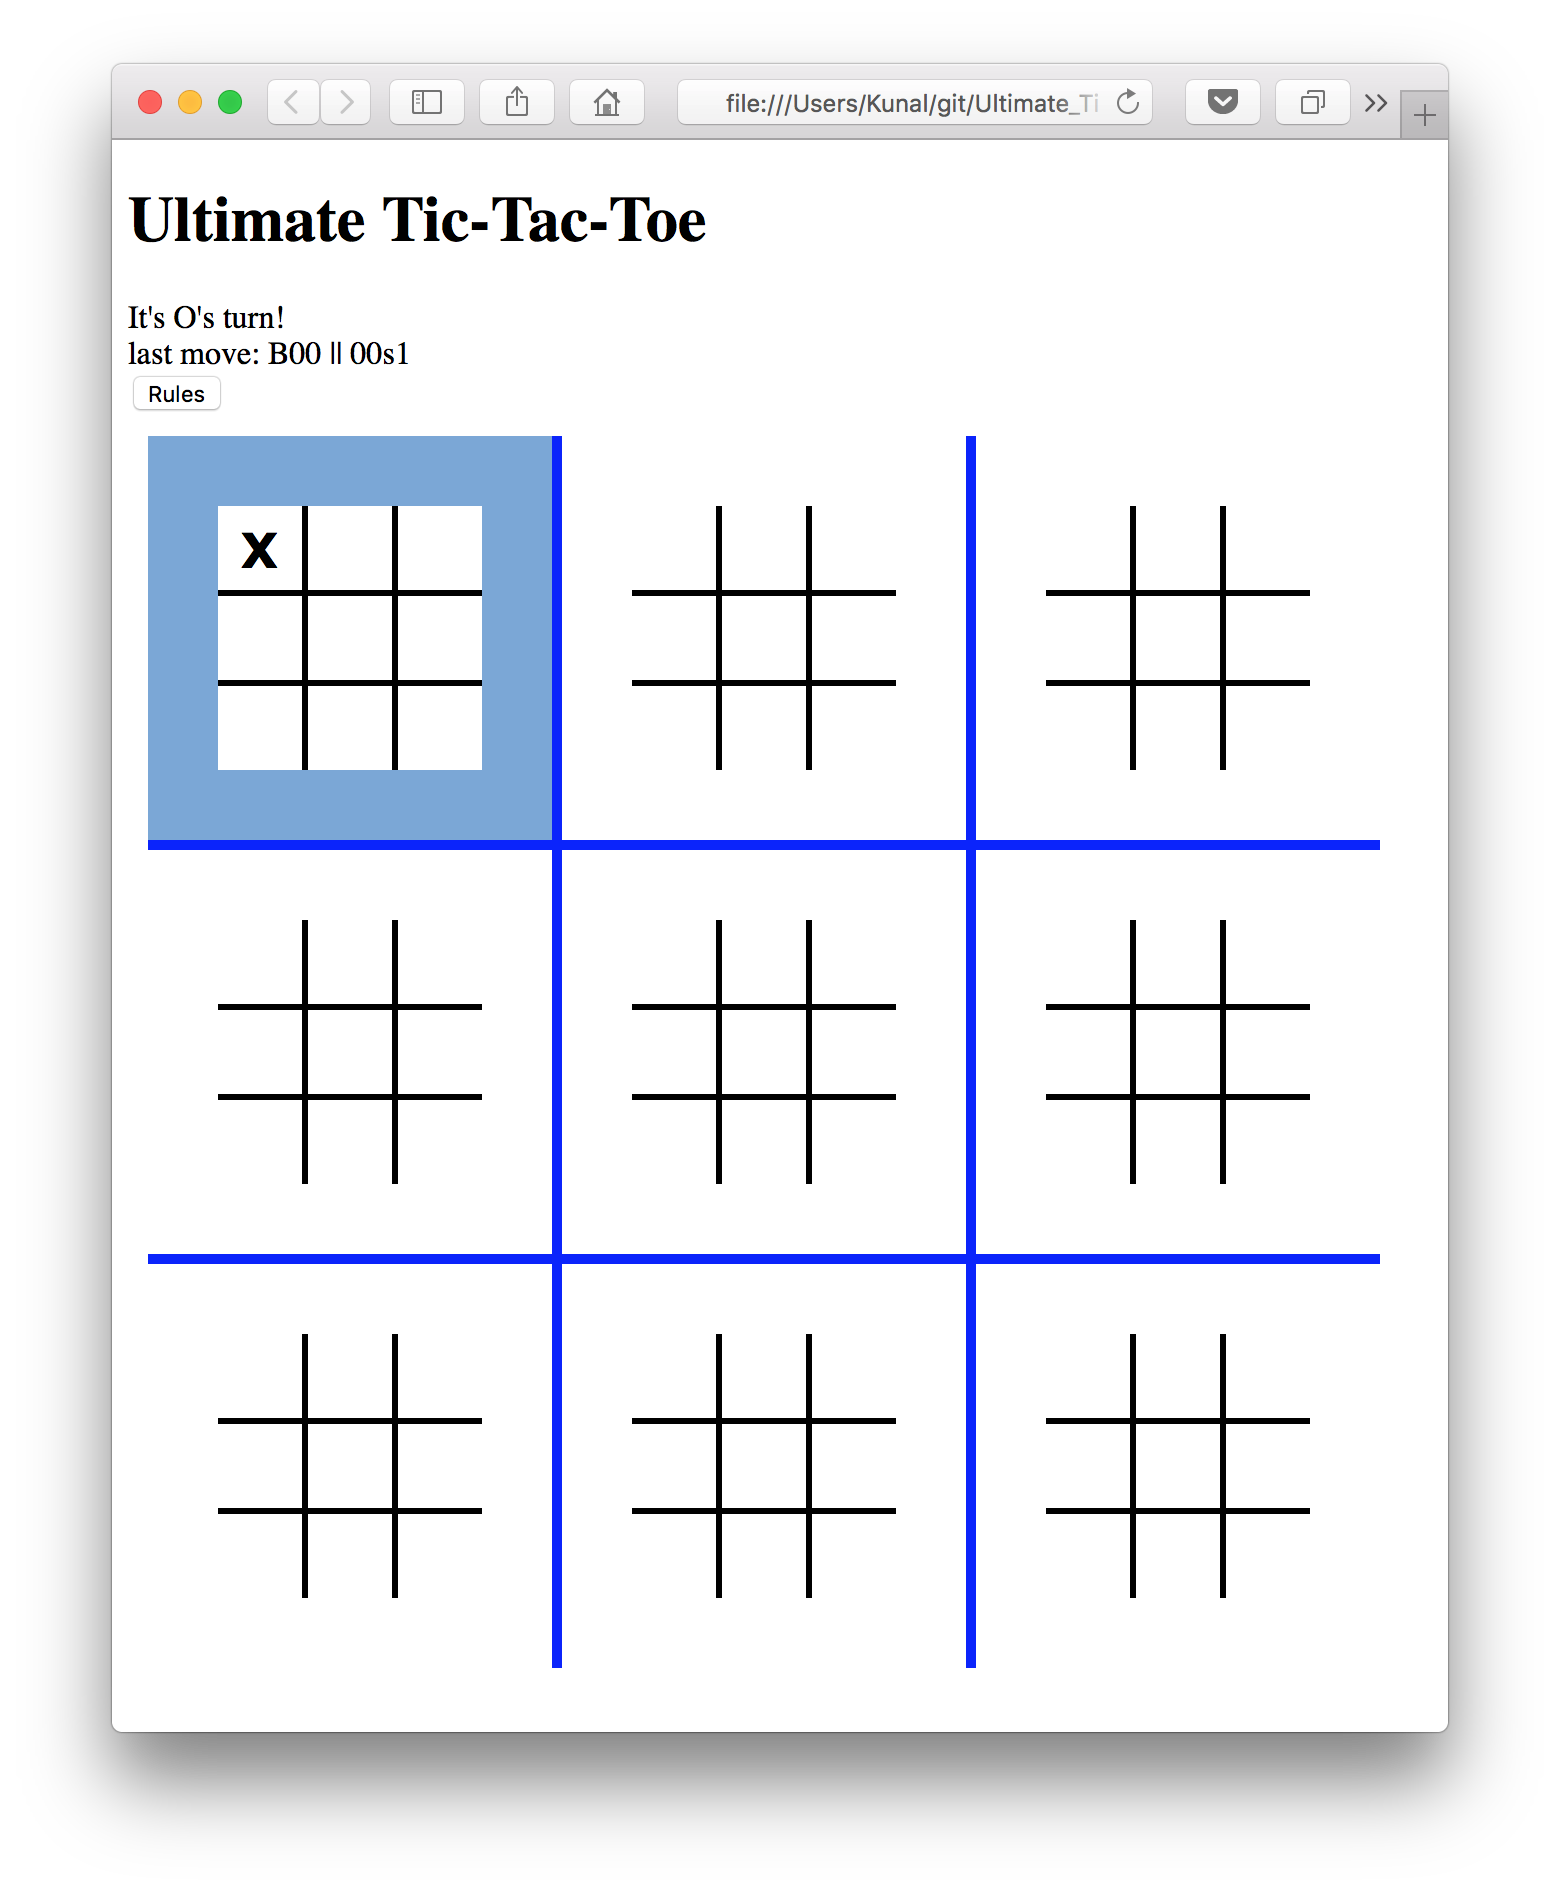
\includegraphics[width=\linewidth]{Figures/Test1-output.png}
  \caption{POC Test 1 Output}
  \label{fig:Test1_output}
\end{figure}

\begin{figure}
  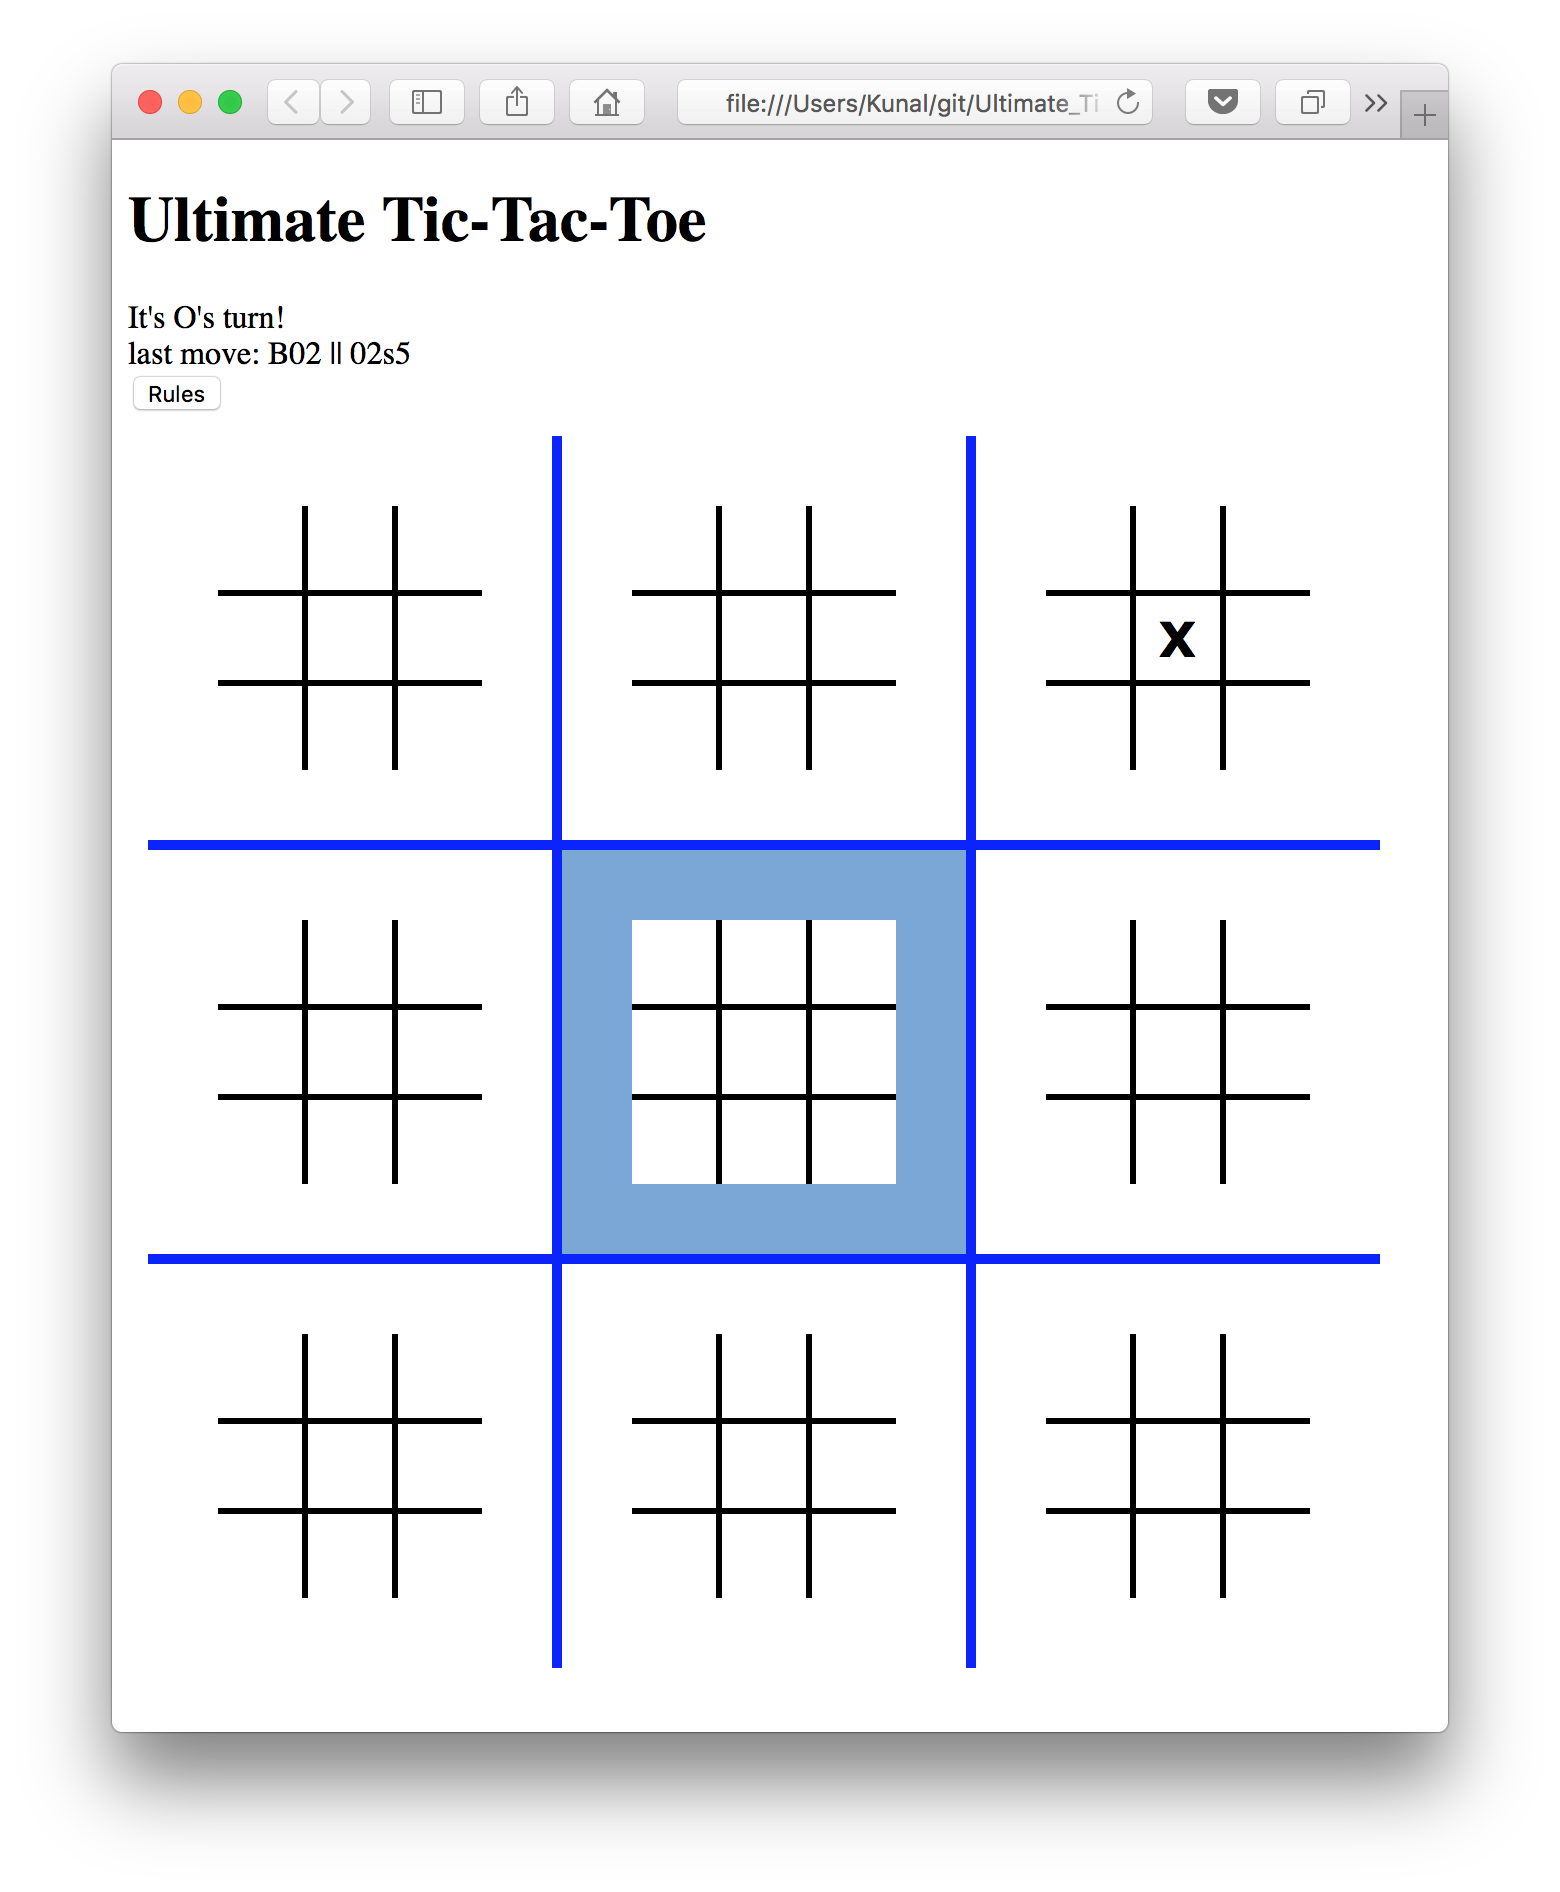
\includegraphics[width=\linewidth]{Figures/Test2-output.png}
  \caption{POC Test 2 Output}
  \label{fig:Test2_output}
\end{figure}

\begin{figure}
  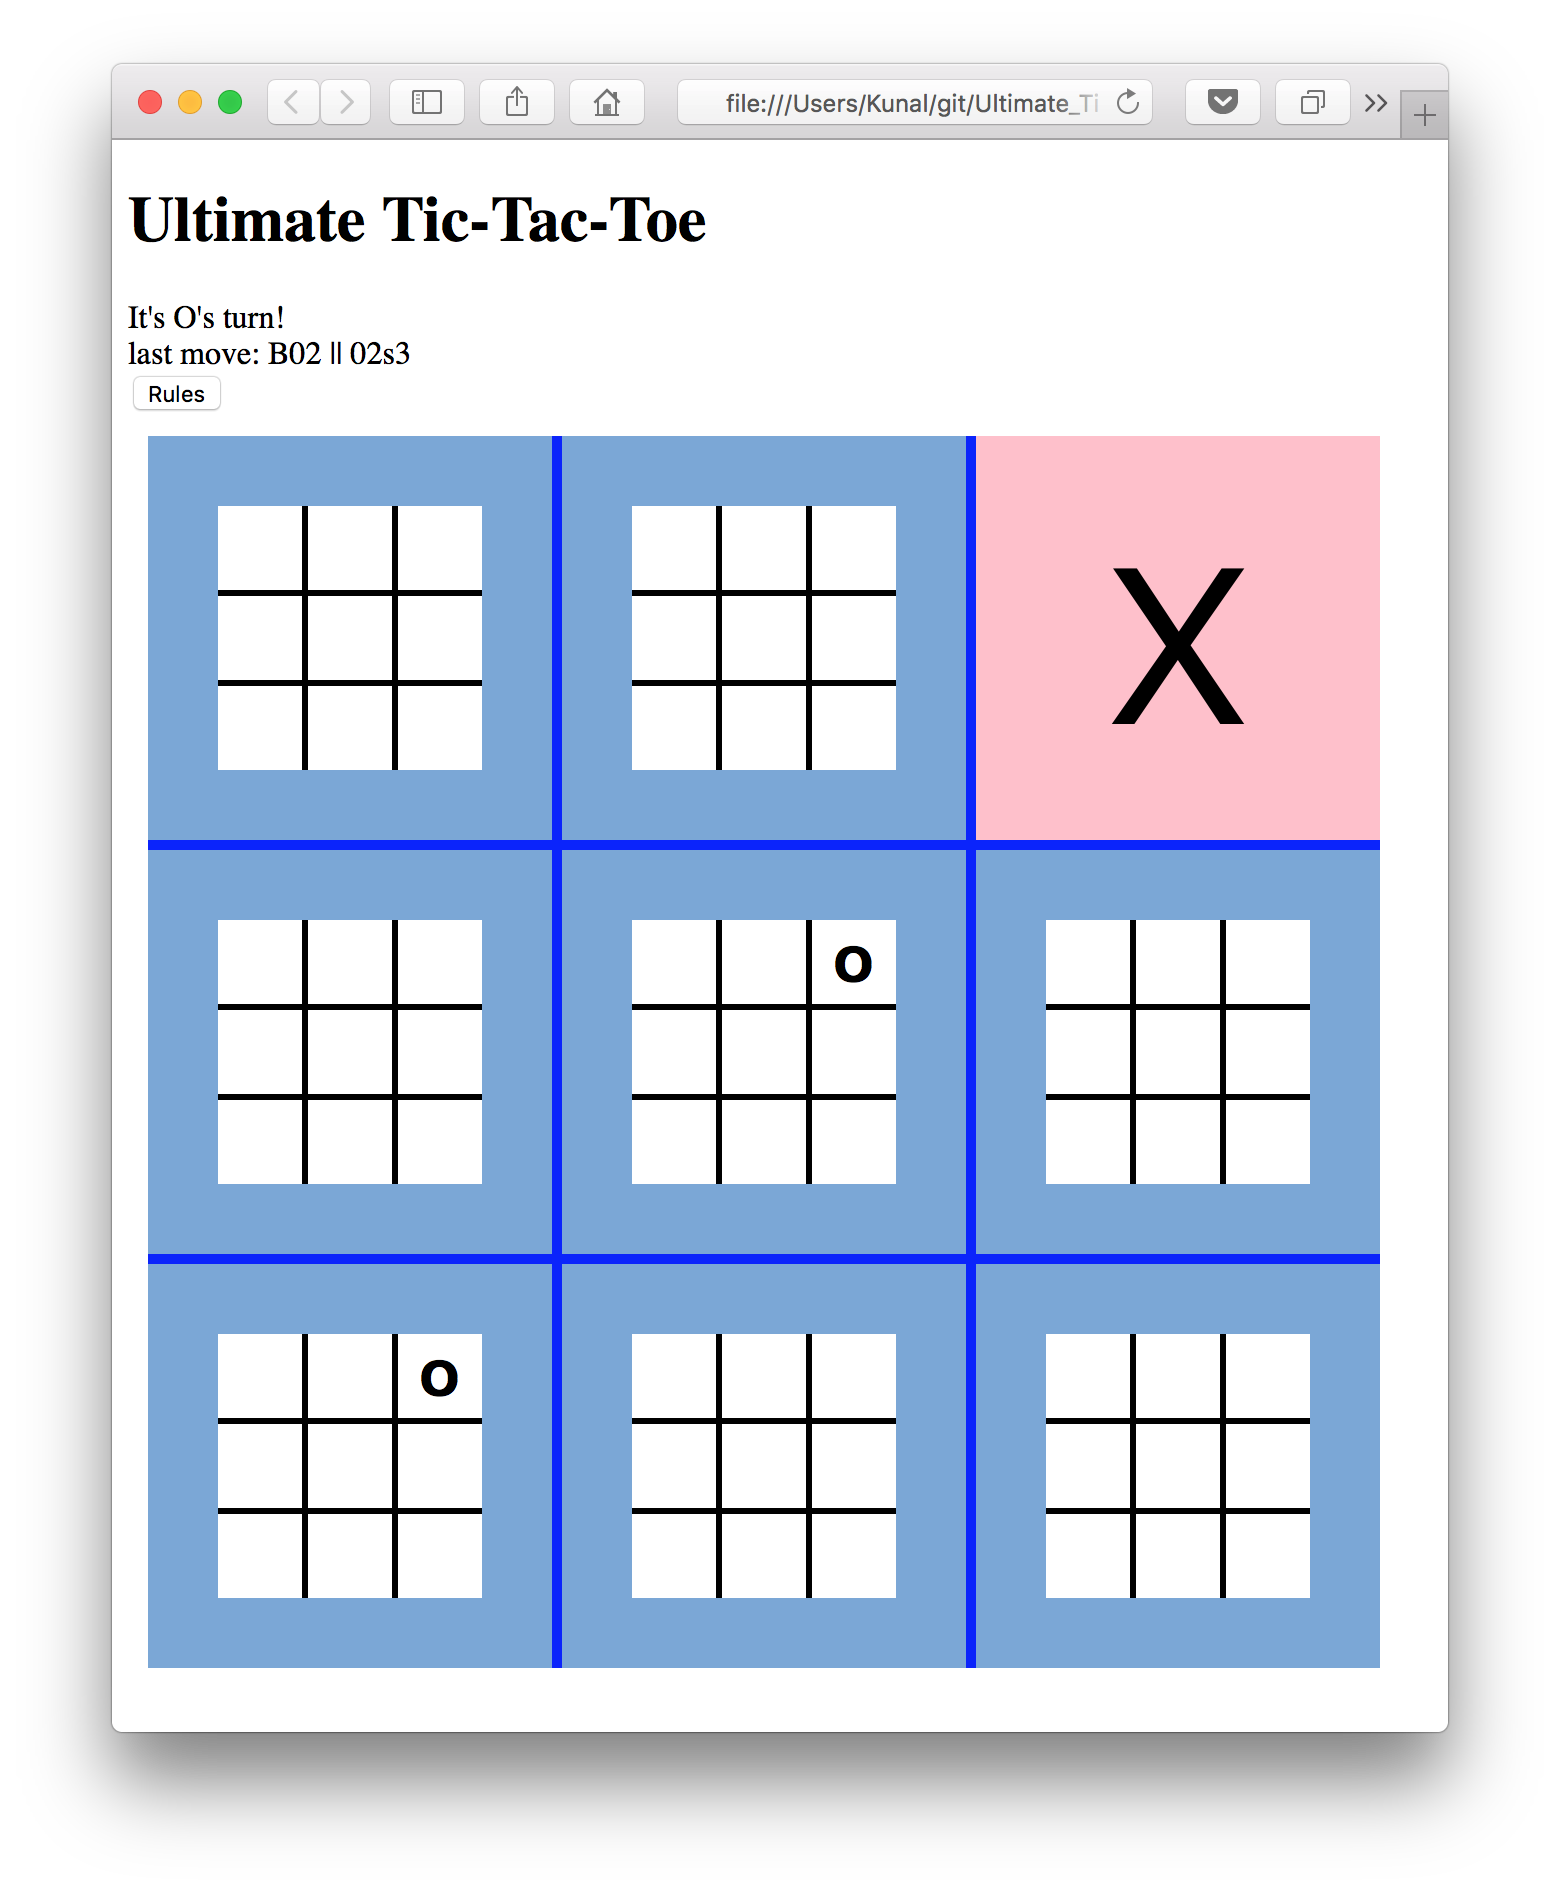
\includegraphics[width=\linewidth]{Figures/Test3-4-output.png}
  \caption{POC Test 3 and Test4 Output}
  \label{fig:Test3_Test4_output}
\end{figure}

\begin{figure}
  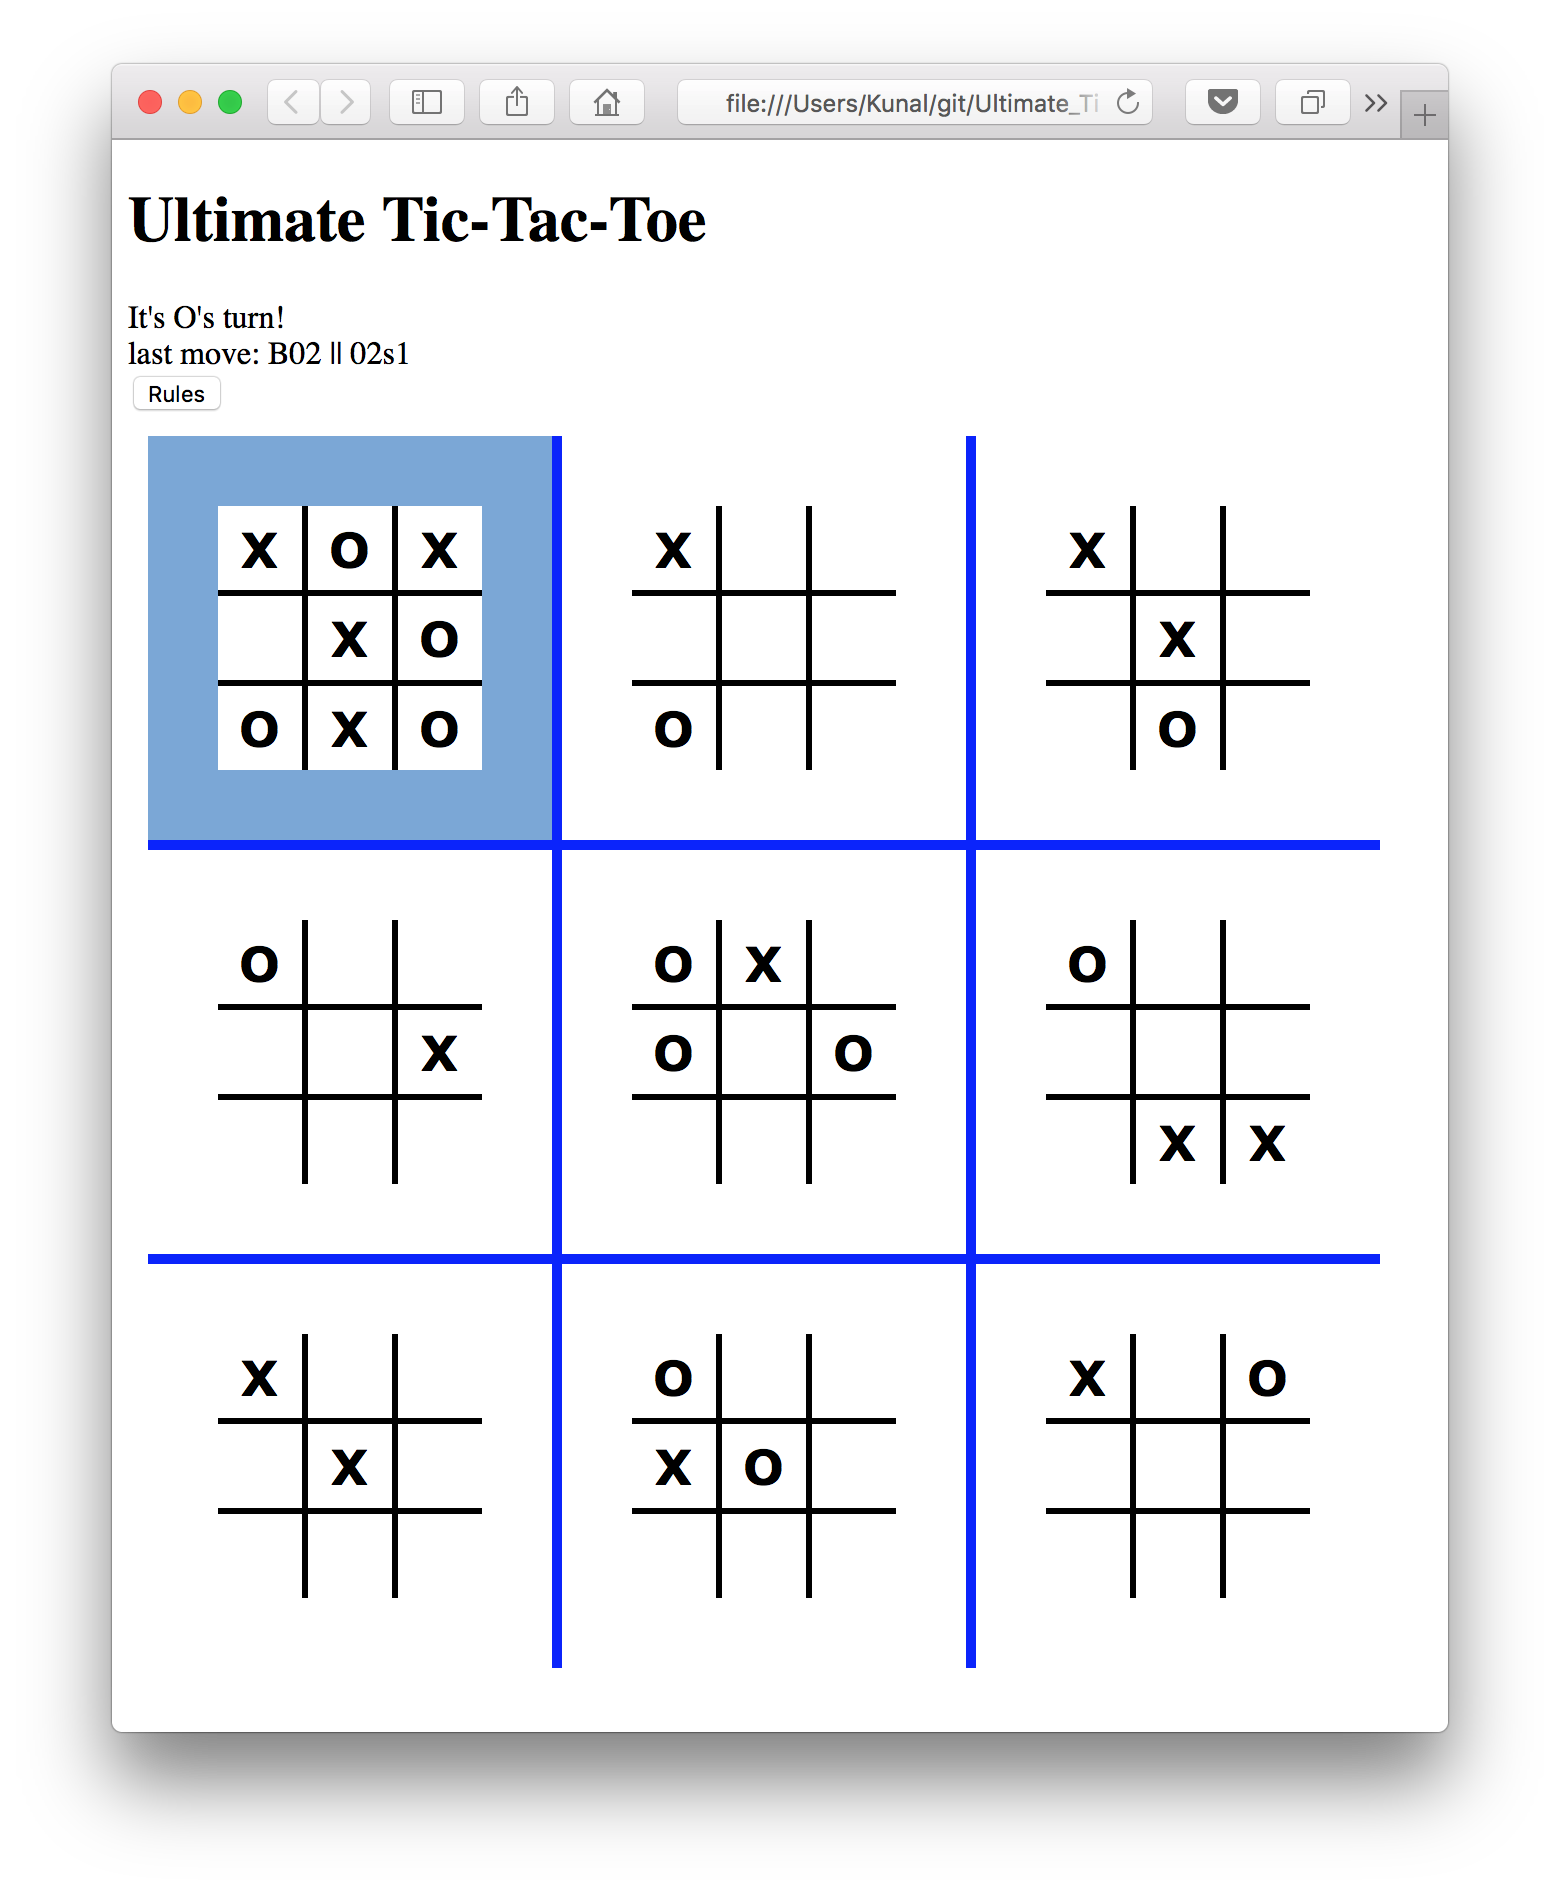
\includegraphics[width=\linewidth]{Figures/Test5-input.png}
  \caption{POC Test 5 Example input}
  \label{fig:Test5_intput}
\end{figure}

\begin{figure}
  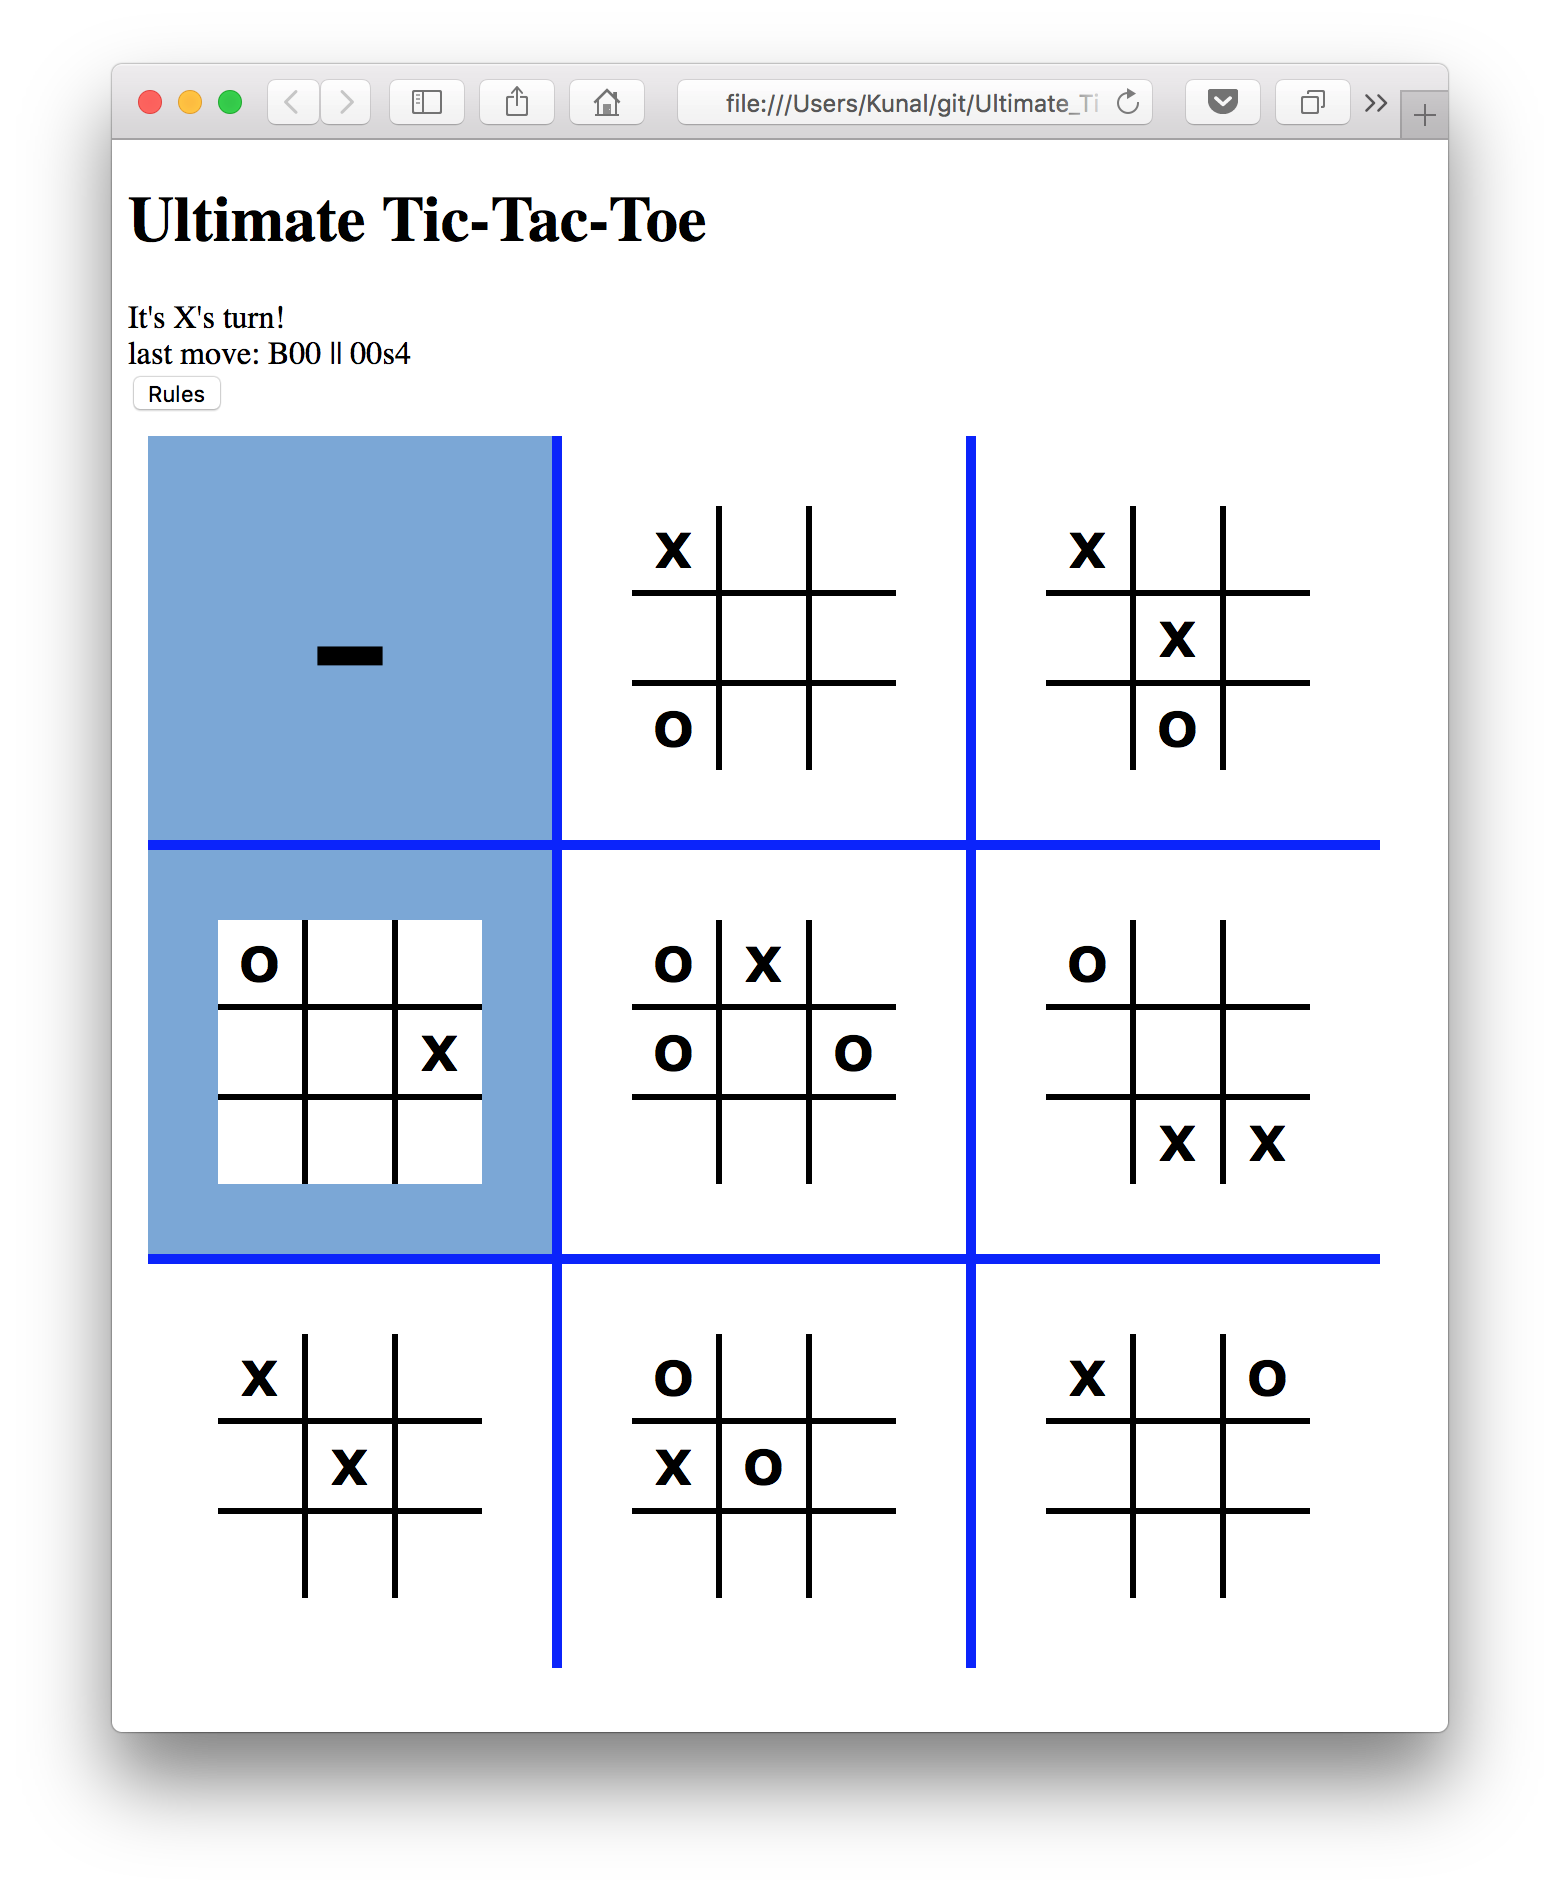
\includegraphics[width=\linewidth]{Figures/Test5-output.png}
  \caption{POC Test 5 Output}
  \label{fig:Test5_output}
\end{figure}

\begin{figure}
  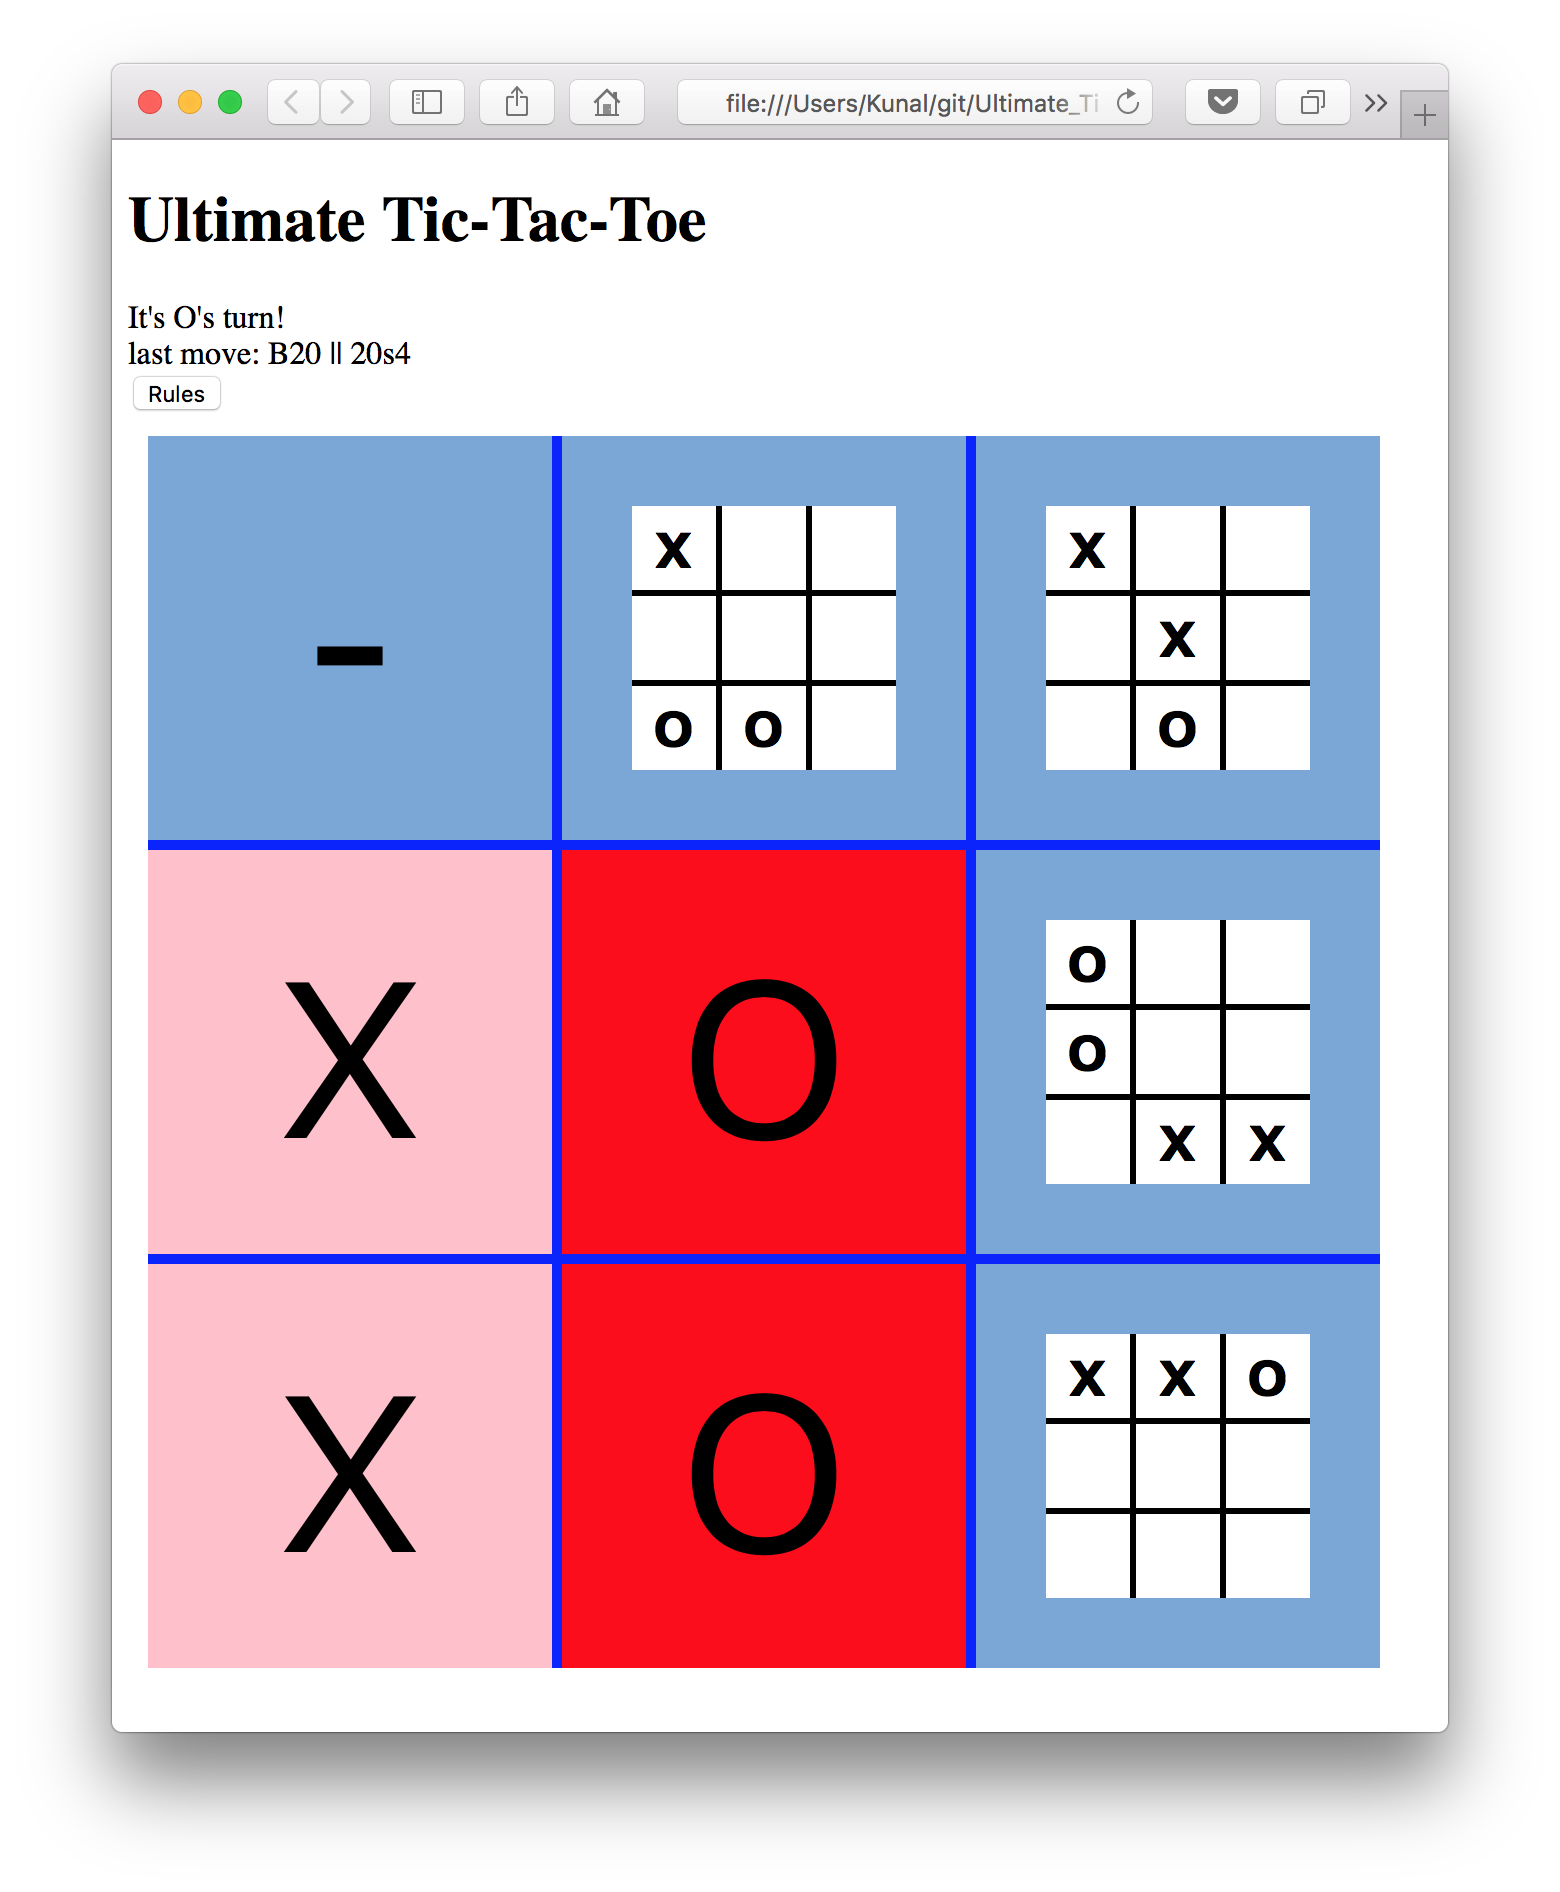
\includegraphics[width=\linewidth]{Figures/Test6-input.png}
  \caption{POC Test 6 Example input}
  \label{fig:Test6_intput}
\end{figure}

\begin{figure}
  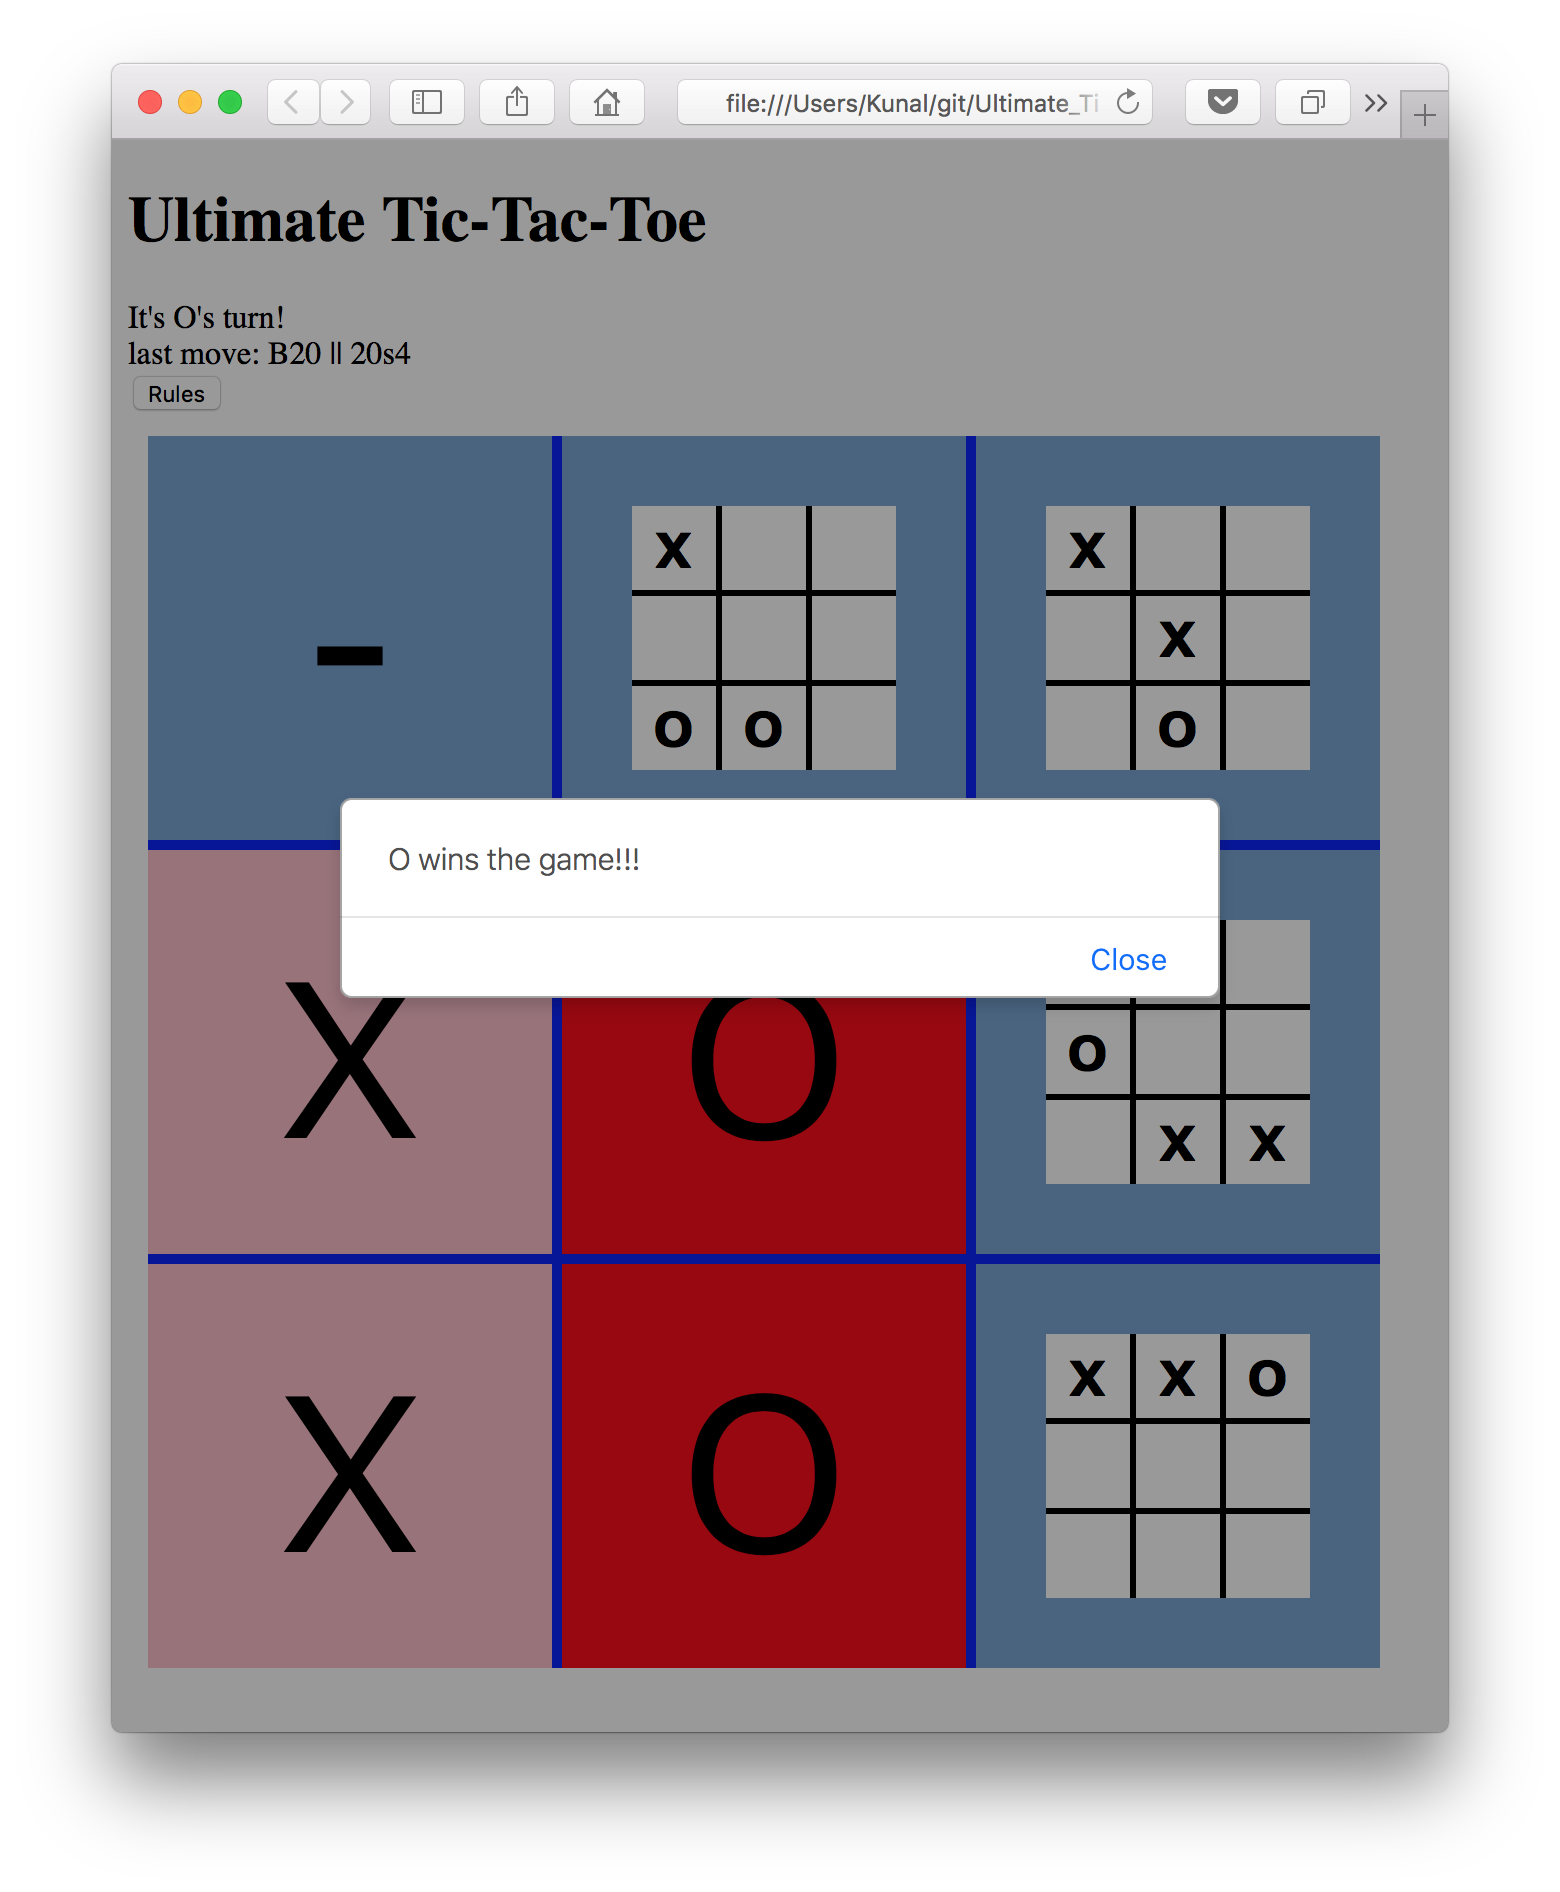
\includegraphics[width=\linewidth]{Figures/Test6-output.png}
  \caption{POC Test 6 Output}
  \label{fig:Test6_output}
\end{figure}

\subsection{Symbolic Parameters}

MAX\_PLAYERS: Maximum number of concurrent players.

\subsection{Usability Survey Questions?}
Answers will be rated from 1 to 5, 5 being the highest
\begin{enumerate}
\item
Is it easy to find the rules of the game? \label{question:q1}
\item
Are the rules easy to understand? \label{question:q2}
\item
Is it clear which player's turn it is? (X or O) \label{question:q3}
\item
Is the color pallet visually appealing? \label{question:q4}
\item
Is the response time satisfying? \label{question:q5}
\item
Was the game able to run on your browser? Please indicate the browser you used
\label{question:q6}
\item
Was the game able to run smoothly on your device. Please indicate the computer
used and the manufactured year \label{question:q7}
\item
Were you offended by anything in the game. Please provide details \label{question:q8}
\item
Did you encounter epileptic symptoms while playing the game \label{question:q9}
\item
Did anything unexpected appear on the screen while playing. Please describe
\label{question:q10}
\item
Is the entire game board visible on the screen? Are there any aspects that are
cut off? Please describe \label{question:q11}


\end{enumerate}

\end{document}